% !TEX root = ../thesis_main.tex



\clearpage
\chapter{Nuclear Physics and Beta Decay Overview}
\label{nuclear_chapter}

\section{The Basics of Beta Decay}
	%\\*
	Standard Model beta decay is well understood.  The Fermi description of beta decay can be found in any nuclear physics textbook, but you have to dig slightly harder to understand Gamow-Teller or mixed decays, all of which are relevant here.  
	
	via Krane~\cite{krane}
	Under the Allowed Approximation, we require that a beta decay may not carry away any orbital angular momentum, because we treat the nucleus as pointlike \aside{Is this even true?  The pointlike thing?  ...No.  No it's not.} and work in the CM frame.  An Allowed decay can, however, change the total nuclear angular momentum, because the outgoing leptons have spin$=1/2$ and therefore carry angular momentum.  Therefore, in an allowed decay, the total nuclear angular momentum must always change by either $0$ or $1$.  
	\note[color=jb]{JB says:  The title of Holstein's review addresses this ``pointlike'' issue, and he describes the ``impulse approximation" in Section V.  The interaction is not pointlike, because all constants are a form factor expansion in $q^2$ -- finite size terms contribute to the Coulomb correction.}
	
	From a 2006 paper by Severijns et al ~\cite{severijns_beck_cuncic_2006}, the selection rules for an allowed transition are:
	
\bea
\Delta I = I_f - I_i = \{0, \pm 1\} \\ 
\hat{\Pi}_i \, \hat{\Pi}_f = +1
\eea

	Then, you can separate the allowed transitions into singlet (anti-parallel lepton spins, $S=0$ -- a Fermi transition) and triplet states (parallel lepton spins, $S=1$ -- a Gamow-Teller transition).
	
	
	Fermi decays are so-called ``vector'' interactions, and happen when the spin of the two leptons involved are antiparallel, so there can be no change in angular momentum (at least in the case of the Allowed approximation).  
	
	Gamow-Teller decays involve two leptons with parallel spins, so the decay must change the projection of the nuclear angular momentum, $M_I$, by exactly one unit (in the case of the Allowed approximation).  They transition may or may not simultaneously change the total nuclear spin, $I$, by one unit.  These are ``axial-vector'' interactions.  (Note that $I=0 \rightarrow I=0$ interactions are never Gamow-Teller decays.  
	
	Probably everything in this section is yoinked from ~\cite{wong1990}, pg 212.  
	
	
%\section{JTW Formalism}	
%	%\\*
%	Describes how to search for a variety of BSM terms within beta decay.  Does not account for certain well-understood effects of similar (or greater) magnitude.
%	
%	% !TEX root = ../thesis_main.tex



% "A PDF for the People"
\bea
\omega(\cdots) \!\!\!\! \!\!\!\! \!\!\!\! \!\!\!\! && \,\,\,\, \,\,\,\, \mathrm{d} \E \, \dOmegae \, \dOmeganu 
\,\, = \,\, \frac{\FF}{(2\pi)^5} \, \pe \Ee (E_0 - \Ee)^2 \dEe \, \dOmegae \, \dOmeganu \, \nonumber\\ 
&&	\times \,\, \xi \left[
	1 + \a \frac{\vecpe\cdot\vecpnu}{\Ee\Enu} + \bFierz \frac{\m c^2}{\Ee} 
%	&& 
    + \,\,  \calign \,\, \Talign(\vecJ) 
	\left(
		\frac{\vecpe \cdot \vecpnu}{3\Ee\Enu}
		- \frac{ (\vecpe\cdot \hatj) (\vecpnu\cdot\hatj) }{\Ee\Enu}
	\right)
	\!
	%\left(
	%	\TalignExpand
	%\right)
\right. \nonumber\\ 
&&	\left. + 
	 \frac{\vecJ}{J} \cdot
	\left(
		\A \frac{\vecpe}{\Ee} 
		+ \B \frac{\vecpnu}{\Enu} 
		+ \D \frac{\vecpe \times \vecpnu}{\Ee\Enu} 
	\right)
\right]
\label{equation:jtw_master}
\eea

%	% equation:jtw_master
%	
%\note{Probably I should now give values for things, or expressions for letters, or something.  }
%We haven't integrated out the neutrino momentum.  Neutrino energy itself is a redundant parameter, I think, because we are already using an endpoint energy and a beta energy, and we are not taking recoil-order effects into account.
%
%For ``convenience'', let's define a nuclear alignment term, $\Talign$, so that:
%\bea
%\Talign(\vecJ) &=& \TalignExpand
%\eea
%
%
%
%\section{Holstein Formalism}
%	An in-depth mathematical description of beta decay, including many smaller effects.  It does not include a description of the BSM physics of greatest interest to us.   Here, we've already integrated over neutrino momentum at least.  That's something.  Here's Holstein's Eq.~(52):
%% !TEX root = ../thesis_main.tex



% "A PDF for the People"
\bea
\mathrm{d}^3 \Gamma &=& 2  G_v^2 \cos^2\theta_c \frac{\FF}{(2\pi)^4} \, \pe \Ee (E_0 - \Ee)^2 \dEe \, \dOmegae 
\nonumber\\
&& \times
\left\{
	F_0(\E) 
	+ \Lambda_1 F_1(\E) \hatn \cdot \frac{\vecpe}{\Ee}
	+ \Lambda_2 F_2(\E) \left[ \left( \nhat \cdot \frac{\vecpe}{\Ee} \right)^2 - \frac{1}{3}\frac{\pe^2}{\Ee^2} \right]
	\right. \nonumber\\ && \left.
	+ \Lambda_3 F_3(\E) 
		\left[ 
			\left( \hatn \cdot \frac{\vecpe}{\Ee} \right)^3
			- \frac{3}{5}\frac{\pe^2}{\Ee^2}\hatn \cdot \frac{\vecpe}{\Ee}
		\right]
\right\}
\label{equation:holstein52}
\eea

%% equation:holstein52
%
%\section{Relation between JTW and Holstein Formalisms}
%	%\\*
%	To conduct a precision search for scalar and tensor couplings, it is necessary to combine the Holstein and JTW models into a single cohesive probability distribution.  
\section{Mathematical Formalism}
	In order to proceed with a measurement, we must find a master equation to describe the probability of beta decay events with any given distribution of energy and momenta among the daughter particles, as a function of the strength of the specific couplings of interest to us.  To do this, two sets of formalisms are combined -- the older formalism from Jackson, Treiman, and Wylde (JTW)~\cite{jtw},~\cite{jtw_coulomb}, which describes the effects of all types of Standard Model and exotic couplings of interest to us here, but which truncates its expression at first order in the (small) parameter of recoil energy, and a newer formalism from Holstein ~\cite{holstein}, which includes terms up to several orders higher in recoil energy, but which does not include any description of the exotic couplings of particular interest to us.  We note that because any exotic couplings present in nature have already been determined to be either small or nonexistant, it is sufficient to describe these parameters with expressions truncated at first order, despite the fact that it is still necessary to describe the larger Standard Model couplings with higher-order terms. 
	
	The procedure for combining the two formalisms is described in detail in Appendix~\ref{appendix_forthepeople}, so we will simply provide the combined master equation here:

\aside{Do it!  Do the master equation!}
%\bea
%\textrm{put  a master equation here.}
%\eea


In the mean time, here's what happens when we integrate JTW over neutrino direction:
% !TEX root = ../thesis_main.tex
%
%
%
% The JTW Proto-Master
\bea
	\textrm{d}^3 \Gamma \dEe \, \dOmegae
	&=& 
	\frac{2}{(2\pi)^4} \, \FF \, \pe \Ee (E_0 - \Ee)^2 \, \dEe \, \dOmegae \, \xi \nonumber\\ 
	&& \times \left[
		1 + \bFierz \frac{\m c^2}{\Ee} + 
		\A  
		\left(
			\frac{\vecJ}{J} \cdot \frac{\vecpe}{\Ee} 
		\right) 
	\right],
\label{equation:integrated_jtw}
\eea
%
where 
\bea
\xi = G_v^2 \, \cos\theta_C \, f_1(E).
\eea



\section{Our Decay}

%  \mbox{ $^{37}\textrm{K} \rightarrow \,^{37}\textrm{\!Ar} + \beta^{+} + \nu_e$ }
\note{ ``Here, we focus on the decay $^{37}\textrm{K} \rightarrow \,^{37}\textrm{\!Ar} + \beta^{+} + \nu_e$.  The angular correlations between the emerging daughter particles provide a rich source of information about the type of interaction that produced the decay.''  }
\note{ ``Of particular interest is the decay process: $^{37}\textrm{K} \rightarrow \,^{37}\textrm{\!Ar} + \beta^{+} + \nu_e$.  Among other useful properties, this is is a `mirror' decay, meaning that the nuclear wavefunctions of the parent and daughter are identical up to their isospin quantum number.  
%the number of protons in the parent nucleus (19) is equal to the number of neutrons in the daughter, and the number of neutrons in the parent (18) is equal to the number of protons in the daughter.  
This property allows us to place strong constraints on the size of the theoretical uncertainties for this decay process within the Standard Model.   %We further exploit this property by noting that both the $^{37}\textrm{K}$ parent and the $^{37}\textrm{\!Ar}$ daughter have nuclear spin $I=3/2$, a fact which is key to this experiment.
''}


Talk about how great \isotope[37]{K} is for what we're doing with it.  Also, drop all the math-numbers to support those assertions.

\missingfigure{This thing is going to need a nuclear level diagram for 37K.  Also, 37K is a really nice isotope for this, because 98\% + 2\%, also because it's a mirror decay, also because it's an alkali.  Also-also, its big $\Abeta$ value means we have a big thing to multiply any $\bFierz$ value there might be when we construct the superratio asymmetry to eliminate systematics.}

\begin{figure}[h!!t]
	\centering
	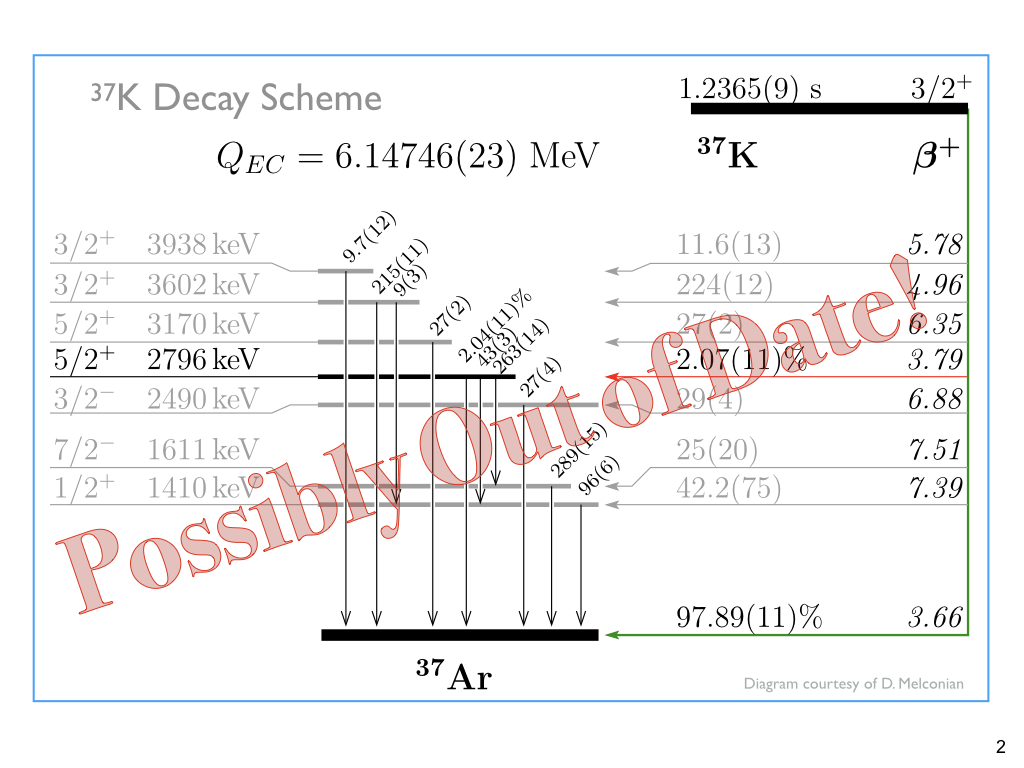
\includegraphics[width=.999\linewidth]
	{Figures/NuclearLevelDiagram_prelim}
	\caption{A level diagram for the decay of $\isotope[37]{K}$.}	
	\label{fig:nuclearleveldiagram}
\end{figure}


\note{Might be worth mentioning about the shake-off electrons too, and how many of them there are.  But then nobody will trust any of the numbers I measured (how did I do that measurement, anyway?), and will want me to just use Dan's that he measured forever ago with a different set of detectors.  (where are those numbers recorded anyway?)  I think I have to mention how many come off and how often at least briefly, because I use the Levinger spectrum for my background modeling.}



